\documentclass{article}

% if you need to pass options to natbib, use, e.g.:
%     \PassOptionsToPackage{numbers, compress}{natbib}
% before loading neurips_2026

% The authors should use one of these tracks.
% Before accepting by the NeurIPS conference, select one of the options below.
% 0. "default" for submission
\usepackage{neurips_2026}
% the "default" option is equal to the "main" option, which is used for the Main Track with double-blind reviewing.
% 1. "main" option is used for the Main Track
%  \usepackage[main]{neurips_2026}
% 2. "position" option is used for the Position Paper Track
%  \usepackage[position]{neurips_2026}
% 3. "eandd" option is used for the Evaluations & Datasets Track
 % \usepackage[eandd]{neurips_2026}
% 4. "creativeai" option is used for the Creative AI Track
%  \usepackage[creativeai]{neurips_2026}
% 5. "sglblindworkshop" option is used for the Workshop with single-blind reviewing
 % \usepackage[sglblindworkshop]{neurips_2026}
% 6. "dblblindworkshop" option is used for the Workshop with double-blind reviewing
%  \usepackage[dblblindworkshop]{neurips_2026}

% After being accepted, the authors should add "final" behind the track to compile a camera-ready version.
% 1. Main Track
 % \usepackage[main, final]{neurips_2026}

% "preprint" option is used for arXiv or other preprint submissions
 % \usepackage[preprint]{neurips_2026}

% to avoid loading the natbib package, add option nonatbib:
%    \usepackage[nonatbib]{neurips_2026}

\usepackage[utf8]{inputenc} % allow utf-8 input
\usepackage[T1]{fontenc}    % use 8-bit T1 fonts
\usepackage{hyperref}       % hyperlinks
\usepackage{url}            % simple URL typesetting
\usepackage{booktabs}       % professional-quality tables
\usepackage{amsfonts}       % blackboard math symbols
\usepackage{amsmath}        % equation, align, etc.
\usepackage{amssymb}        % \mathbb, \mathcal, etc.
\usepackage{nicefrac}       % compact symbols for 1/2, etc.
\usepackage{microtype}      % microtypography
\usepackage[table]{xcolor}  % colors + \rowcolor for tables
\usepackage{multirow}       % \multirow in tables
\usepackage{enumitem}       % itemize/enumerate with [leftmargin=...] options


\title{DUET: Principled Experience Replay for LLM Agent Reinforcement Learning}


% The \author macro works with any number of authors. There are two commands
% used to separate the names and addresses of multiple authors: \And and \AND.
%
% Using \And between authors leaves it to LaTeX to determine where to break the
% lines. Using \AND forces a line break at that point. So, if LaTeX puts 3 of 4
% authors names on the first line, and the last on the second line, try using
% \AND instead of \And before the third author name.


\author{%
  Anonymous Authors\\
  % --- For final/camera-ready, replace with:
  % Author Name\thanks{Acknowledgement note.} \\
  % Affiliation\\
  % \texttt{email@institution.edu} \\
}


\begin{document}


\maketitle


% ============================================================================
% Abstract
% ============================================================================
% ============================================================================
% Abstract — DUET (NeurIPS 2026)
% Word count: ~211 words (target 180-220)
% Last revised: 2026-05-04 (v2 — rewrite for readability)
% ============================================================================
%
% Design principles for this version:
%   - Open with plain English, not jargon. The 1.5B success-rate numbers
%     come in sentence 1 as a concrete hook.
%   - Each sentence carries ONE idea. No subordinate-clause stacks.
%   - "Exploration is punished." stands alone as a 3-word punch line.
%   - DR3 / BC / SC / Action / State are NOT named in the abstract;
%     they are introduced in the body. Abstract uses plain descriptions.
%   - Em-dash used only once (--- around "experience replay" definition).
%   - Final sentence carries both aggregate (+13pp) and worst-case (+17.5pp).
% ============================================================================

\begin{abstract}
Experience replay from strong teacher agents is an appealing way to overcome the cold-start problem in on-policy RL for LLM agents. Yet in GRPO-style updates, inserting replayed teacher trajectories into the same rollout batch as student trajectories is not a benign form of supervision: it changes both the advantage estimates and the distributional assumptions underlying the policy gradient. We identify two systematic biases induced by this teacher-mixing replay. First, successful teacher rollouts contaminate the group baseline, suppressing the advantages assigned to successful on-policy student rollouts and thereby discouraging exploration. Second, teacher trajectories are off-policy, but exact teacher--student importance correction can be infeasible when teacher likelihoods are unavailable, leaving standard GRPO updates with an uncorrected distribution mismatch. Therefore, we propose \textbf{DUET}, a principled experience-replay framework that first corrects these biases through baseline separation and density-ratio correction, and then extracts complementary teacher signals through two channels: token-level behavior cloning in the action channel and potential-based state-progress shaping in the state channel. Together, these components let DUET exploit teacher trajectories beyond direct replay while adaptively attenuating teacher influence as the student improves, turning teacher data into complementary signals for action imitation and state-guided exploration. Across ALFWorld and WebShop with two model scales, DUET achieves the best performance in all used settings, improving the strongest prior baseline by 13.0 percentage points on average and by 17.5 points in the weakest-agent regime. Code is available at \url{https://anonymous.4open.science/r/DUET-DC26}.
\end{abstract}


% ============================================================================
% Section 1: Introduction
% ============================================================================
% ============================================================================
% Introduction — DUET (NeurIPS 2026)
% Last revised: 2026-05-04
%
% Structure: 5-paragraph diagnose-then-fix arc
%   §1 Problem    — cold-start trap of on-policy RL on weak LLM agents
%   §2 Existing   — LUFFY/CHORD as natural mitigations, with CHORD's known critique
%   §3 Diagnosis  — TWO systematic biases (paper's intellectual contribution)
%   §4 DUET       — principled fix + extensions, two-channel architecture
%   §5 Results    — 4/4 SOTA, +13pp avg, contributions list
%
% Citation placeholders: \citep{TODO_*} need bibtex entries:
%   - GRPO: shao2024deepseekmath
%   - LUFFY: yan2025luffy (placeholder)
%   - CHORD: chord2025 (placeholder)
%   - ALFWorld: shridhar2021alfworld
%   - WebShop: yao2022webshop
%   - Ng potential shaping: ng1999policy
%   - GAN density ratio: goodfellow2014gan, sugiyama2012density
% ============================================================================

\section{Introduction}

% --- Paragraph 1: Problem statement ---
Training large language model (LLM) agents to interact with complex environments via reinforcement learning has emerged as a central paradigm for embodied and tool-using AI~\citep{TODO_alfworld,TODO_webshop,TODO_react}. On-policy methods such as GRPO~\citep{TODO_grpo} train the agent purely from its own rollouts and provide stable updates when the policy is already capable. On weaker base models, however---the regime most relevant to deployment cost---on-policy RL hits a \emph{cold-start trap}: success rates collapse to near zero before the policy has accumulated enough successful trajectories to bootstrap learning. On ALFWorld~\citep{TODO_alfworld} and WebShop~\citep{TODO_webshop}, GRPO on Qwen2.5-1.5B-Instruct reaches only $1.0\%$ and $0.5\%$ strict success rates respectively, with no recovery within $100$ training steps.

% --- Paragraph 2: Existing teacher-mixing approaches ---
A natural mitigation is to inject expert trajectories from a stronger teacher LLM into the rollout batch, as in LUFFY~\citep{TODO_luffy} and CHORD~\citep{TODO_chord}. These methods provide cold-start guidance and demonstrate substantial gains over pure on-policy RL on weak agents. However, both approaches treat teacher trajectories as if they were on-policy samples, plugging them directly into the GRPO objective with at most a manually-scheduled imitation weight (CHORD). This design choice has drawn criticism in prior reviews, both for its heuristic nature and for unstable late-training dynamics.

% --- Paragraph 3: Diagnosis (the paper's intellectual contribution) ---
We identify two \emph{systematic biases} in LUFFY-style experience replay that explain these issues:
\begin{itemize}[leftmargin=1.5em, itemsep=2pt, topsep=2pt]
\item \textbf{Baseline contamination.} GRPO normalizes advantages by the within-group mean and standard deviation. Teacher trajectories are always successful (reward $=1$); when they share a group with on-policy rollouts, they inflate the group's baseline. As a consequence, even \emph{successful} on-policy rollouts can receive negative advantage, and the policy gradient effectively penalizes the very exploration that on-policy RL is trying to encourage.
\item \textbf{Unaddressed off-policy mismatch.} Teacher trajectories are sampled from a distribution $\pi_\beta \neq \pi_\theta$, so the policy-update importance ratio for teacher samples is biased. Without explicit correction, teacher gradients continue to dominate even after the student has matched the teacher's capability---damaging asymptotic performance and forcing practitioners to hand-tune teacher-decay schedules.
\end{itemize}
Both biases compound on weak base models, where the gap between teacher and student is largest and lasts longest---which is exactly where one most wants teacher mixing to work.

% --- Paragraph 4: Our solution: DUET ---
We propose \textbf{DUET}, a principled experience-replay framework that addresses both biases and extracts richer signal from teacher data through two complementary channels.
\begin{itemize}[leftmargin=1.5em, itemsep=2pt, topsep=2pt]
\item \textbf{Fix~1 --- Baseline separation.} GRPO baselines are computed separately for teacher and on-policy sub-groups, eliminating the contamination bias.
\item \textbf{Fix~2 --- DR3 density-ratio correction.} A small discriminator $D(\cdot)$ estimates the importance ratio $\hat w(\tau) = \pi_\theta/\pi_\beta$ for teacher trajectories; this replaces the (biased) GRPO importance ratio for teacher samples. By construction, $\hat w \to 1$ as the student catches up, providing data-driven teacher fade-out without any schedule.
\item \textbf{Extension~1 --- BC adaptive imitation.} A token-level cross-entropy loss on teacher tokens with adaptive weight $\mu(t)$ serves as a \emph{cold-start safety net} while DR3's discriminator is still learning. The weight $\mu(t)$ decays as discriminator accuracy rises, transferring control to DR3 once the latter is reliable.
\item \textbf{Extension~2 --- SC potential-based shaping.} A hash-based expert progress map $P(s)$ provides per-state reward shaping for on-policy samples only, using the potential-based form $r' = r + \beta\bigl(P(s')-P(s)\bigr)$ that preserves the optimal policy by Ng et al.~\citeyearpar{TODO_ng1999}.
\end{itemize}
The four mechanisms are organized into two orthogonal channels: an \textbf{Action Channel} (DR3 + BC) operating on the policy gradient, and a \textbf{State Channel} (SC) operating on the reward. Every teacher mechanism is driven by an internal, data-derived signal---no manual schedule.

% --- Paragraph 5: Results & contributions ---
Across four settings spanning two model sizes (Qwen2.5-1.5B/3B-Instruct) and two environments (ALFWorld, WebShop), DUET achieves state-of-the-art on every setting, surpassing the strongest baseline (CHORD or SFT$+$GRPO) by $+13.0$pp success rate on average. The improvement is largest on weak base models ($+17.5$pp on 1.5B), confirming that DUET specifically resolves the cold-start regime where on-policy RL fails. Component ablations show that each of the four mechanisms contributes non-trivially, and that the two channels are complementary rather than redundant. Our contributions are:
\begin{enumerate}[leftmargin=1.5em, itemsep=1pt, topsep=2pt]
\item A \textbf{diagnosis} of two systematic biases---baseline contamination and unaddressed off-policy mismatch---in LUFFY-style experience replay for LLM agents.
\item \textbf{DUET}, a principled experience-replay framework with four self-calibrating mechanisms organized into two orthogonal channels.
\item \textbf{Strong empirical results}: SOTA on all four (model size $\times$ environment) settings, with $+13.0$pp average success-rate gain over the strongest non-DUET baseline, and up to $+17.5$pp on weaker base models.
\end{enumerate}



% ============================================================================
% Section 2: Related Work
% TODO: write related-work section. Should cover:
%   - On-policy RL for LLM agents (GRPO, RLHF lineage, ReAct-style frameworks)
%   - Teacher mixing / experience replay (LUFFY, CHORD)
%   - Distillation and density-ratio methods
%   - Reward shaping in RL (Ng et al. 1999 and follow-ups)
% ============================================================================
% % ============================================================================
% Related Work — DUET (NeurIPS 2026)
% Rewritten to foreground teacher replay, estimator bias, and dual-channel use
% of demonstrations while keeping the section compact.
% ============================================================================

\section{Related Work}

\paragraph{Group-based RL for interactive LLM agents.}
LLM agents are increasingly trained in multi-turn, sparse-reward environments~\citep{shridhar2020alfworld,yao2022webshop,yao2022react}. GRPO~\citep{shao2024deepseekmath}, building on PPO~\citep{schulman2017ppo} and RLHF~\citep{ouyang2022training}, replaces a learned critic with group-relative rewards and has become a practical backbone. Recent agent-RL work adds unified environments~\citep{xi2024agentgym}, stability analysis~\citep{wang2025ragen}, and finer-grained credit assignment~\citep{feng2025gigpo}. DUET is complementary to these on-policy advances: it studies how cached teacher trajectories should enter a GRPO-style update without corrupting on-policy credit.

\paragraph{Teacher replay beyond imitation.}
Demonstrations have long been used for cold-start exploration in imitation, demonstration-augmented, and offline-to-online RL~\citep{ross2011dagger,hester2018deep,nair2020awac,kostrikov2022iql}. For LLM post-training, LUFFY mixes off-policy reasoning traces with on-policy GRPO rollouts~\citep{yan2025luffy}, while CHORD reframes SFT as a dynamically weighted auxiliary objective inside on-policy RL~\citep{zhang2025chord}. These methods show that expert data helps weak learners, but mainly use teacher trajectories as action or token sequences. DUET instead treats demonstrations as structured interaction experience: teacher actions provide a corrected replay signal, while teacher states provide progress guidance.

\paragraph{Correcting off-policy teacher actions.}
Direct teacher mixing is not benign supervision inside group-normalized policy gradients. Successful teacher rollouts can shift the group baseline, and teacher actions are off-policy. Classical off-policy policy gradients therefore motivate behavior--target correction~\citep{degris2012offpolicy}. When exact teacher likelihoods are unavailable, density-ratio estimation is a standard surrogate~\citep{sugiyama2012density}; binary classifiers estimate distributional differences in generative modeling and adversarial imitation~\citep{goodfellow2014generative,ho2016gail}. DUET applies this principle narrowly: a discriminator-based replay weight approximates teacher--student correction, while baseline separation prevents teacher rewards from suppressing on-policy successes.

\paragraph{State progress and reward shaping.}
Teacher trajectories also contain environment states, not only output actions. In ALFWorld and WebShop, intermediate observations can reveal progress toward household or product-search goals~\citep{shridhar2020alfworld,yao2022webshop}. Reward shaping offers a natural lens: potential-based shaping preserves optimal policies under $F=\gamma\Phi(s')-\Phi(s)$~\citep{ng1999policy}. DUET uses a coarser empirical progress potential built from successful teacher state visitation. The bonus is applied only to on-policy rollouts, keeping state guidance separate from corrected teacher-action replay.



% ============================================================================
% Section 3: Method
% ============================================================================
% ============================================================================
% Method — DUET
% ============================================================================

\section{DUET: Dual-Channel Teacher Utilization}
\label{sec:method}

\subsection{Setup}
\label{sec:setup}

We train a student policy $\pi_\theta(a\mid s)$ with GRPO~\citep{shao2024deepseekmath} in sparse-reward interactive environments.
For each task, the student samples $n_o$ on-policy rollouts $G^o$.
We also use a fixed cache of successful trajectories $\{\tau^\beta\}$ collected from a stronger teacher policy $\pi_\beta$.
Following teacher-mixed replay~\citep{yan2025luffy, zhang2025chord}, each training group includes $n_\beta$ teacher trajectories $G^\beta$:
\begin{equation}
G = G^o \cup G^\beta,
\qquad
|G| = n_o+n_\beta .
\label{eq:mixed_group}
\end{equation}
Our goal is to use this cache without letting off-policy teacher trajectories distort the group-normalized policy-gradient update.

\subsection{Overview}
\label{sec:overview}

\begin{figure}[t]
\centering
\IfFileExists{figures/fig1_method.pdf}{%
  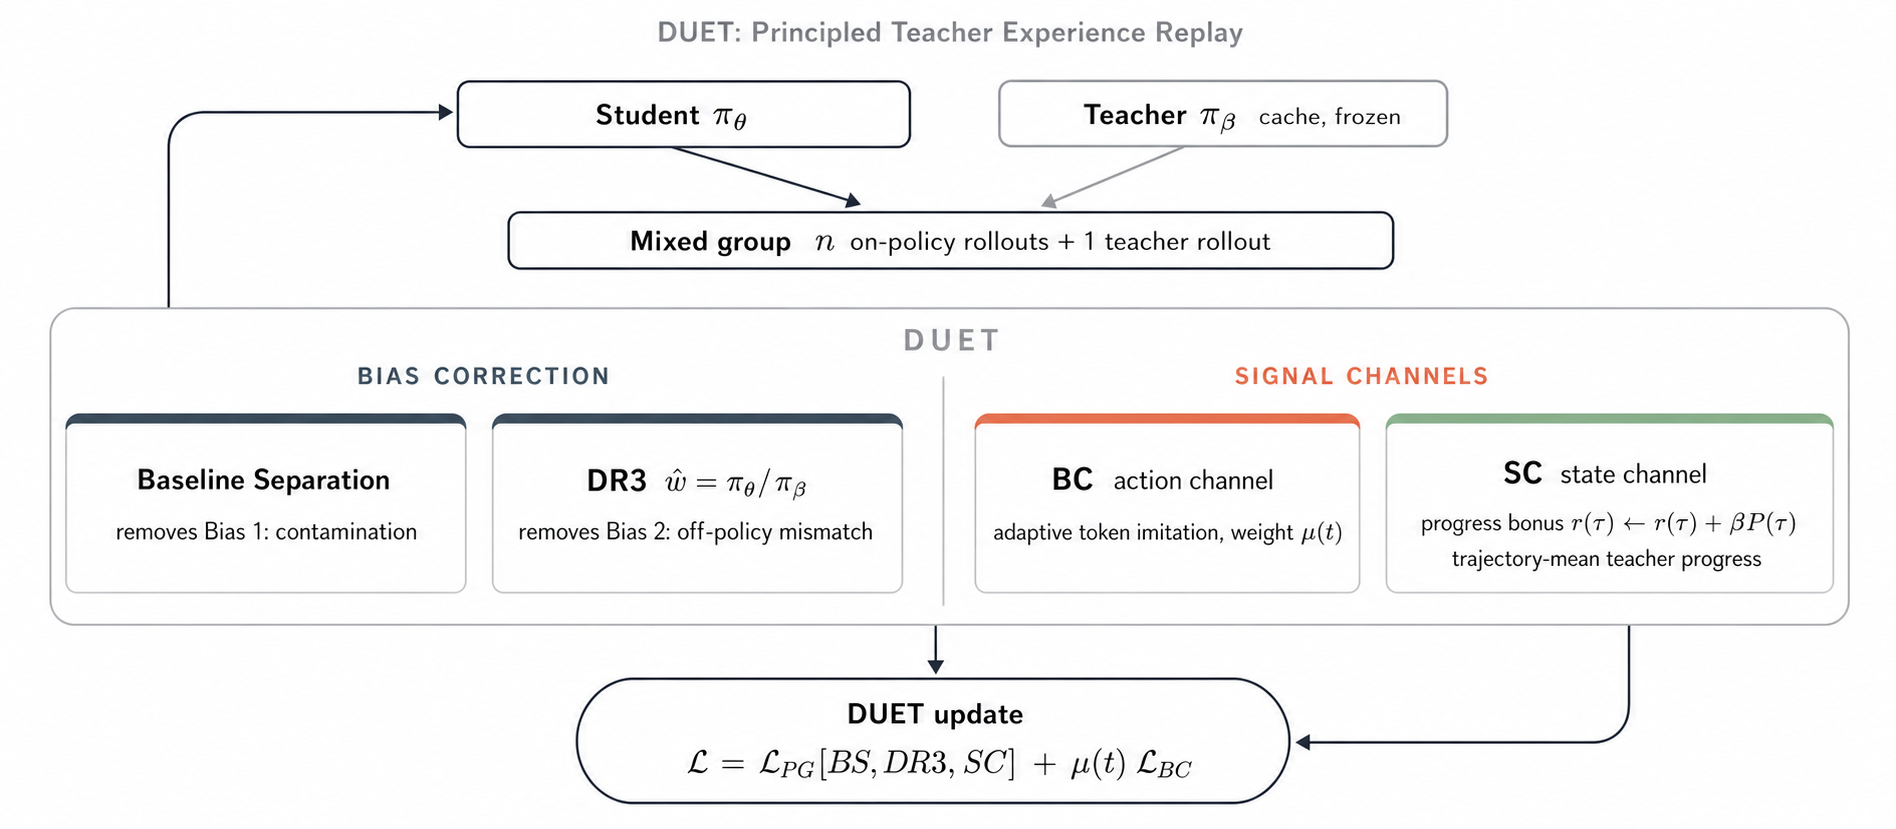
\includegraphics[width=0.95\linewidth]{figures/fig1_method.pdf}%
}{\IfFileExists{figures/fig1_method.png}{%
  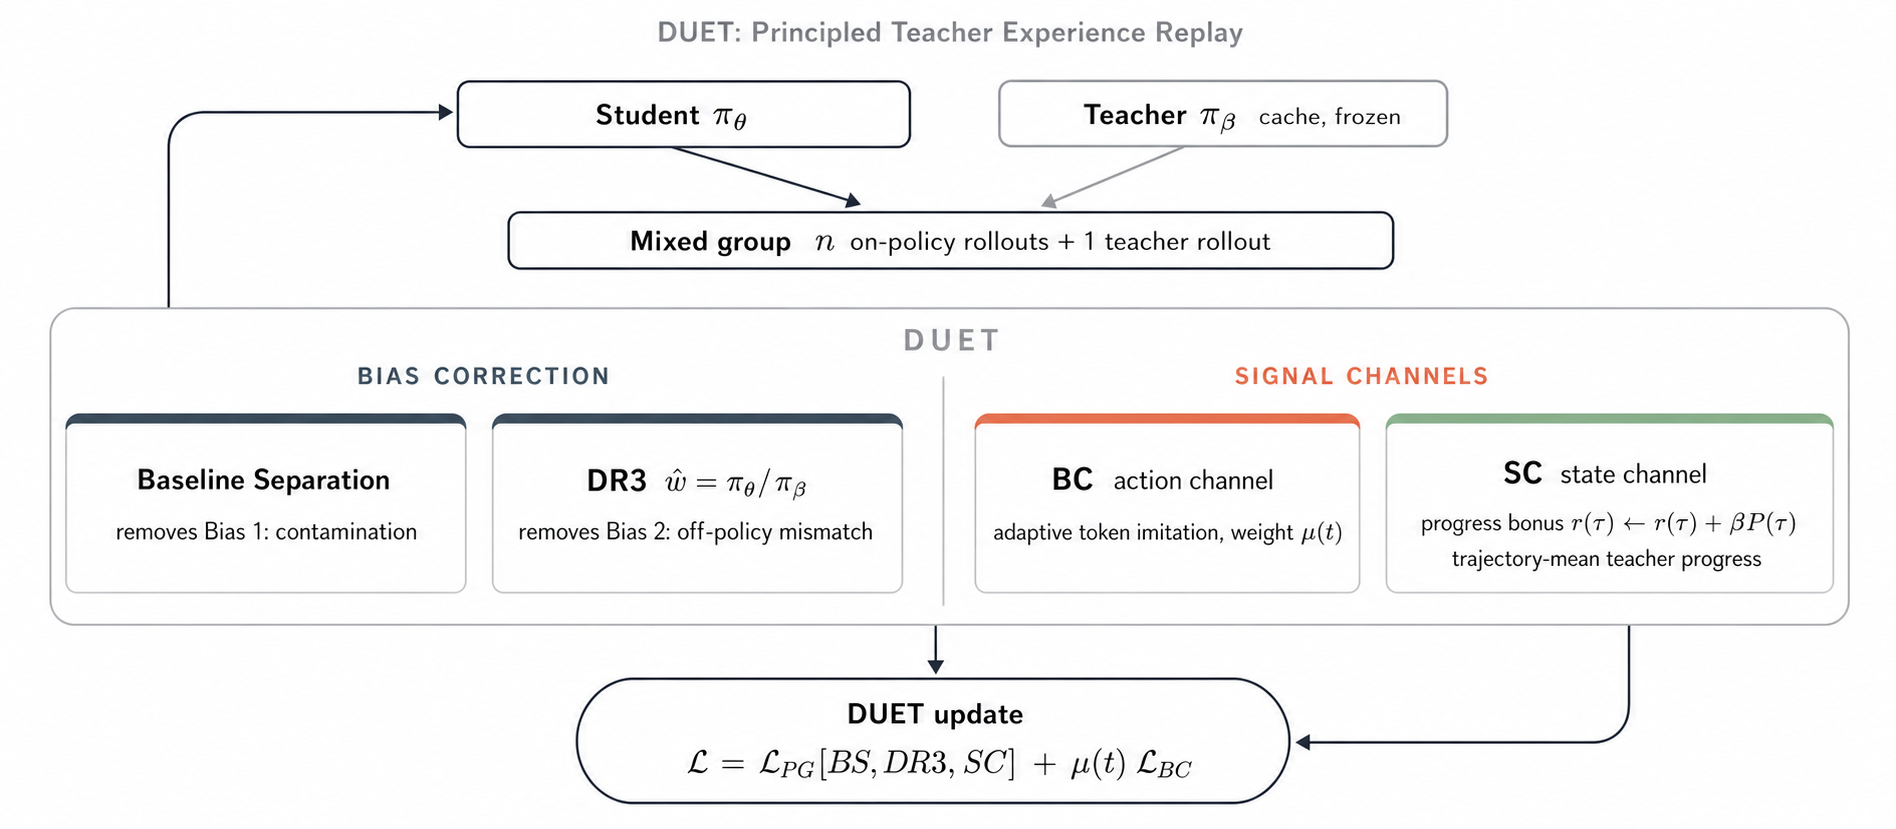
\includegraphics[width=0.95\linewidth]{figures/fig1_method.png}%
}{\IfFileExists{figures/fig1_method.jpg}{%
  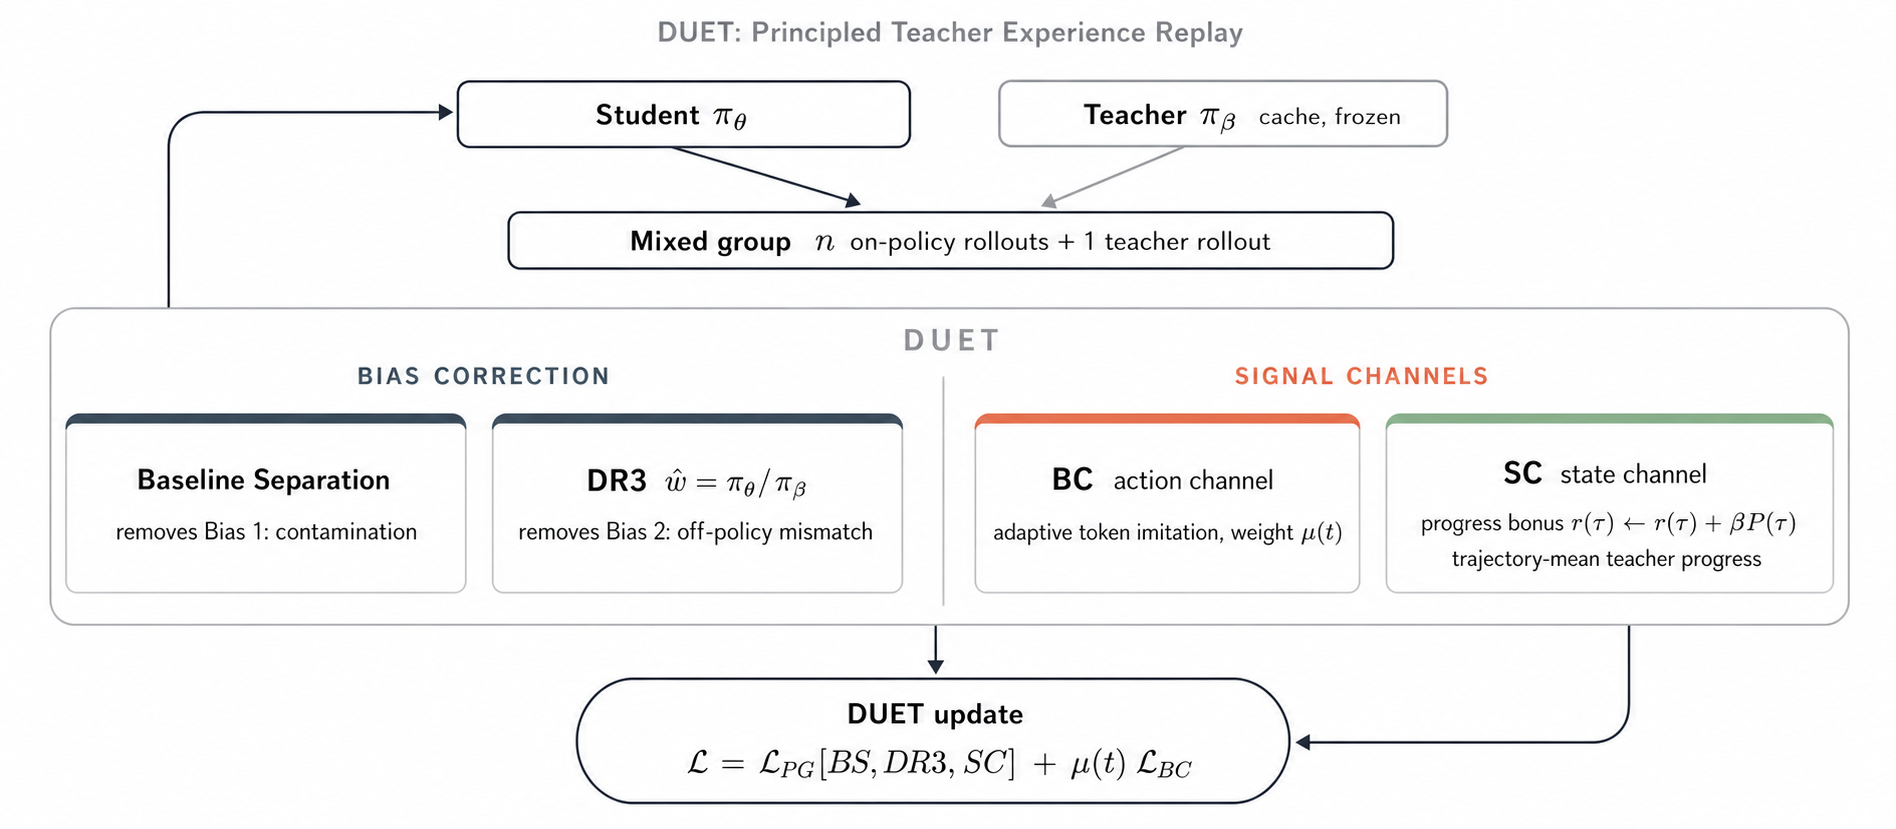
\includegraphics[width=0.95\linewidth]{figures/fig1_method.jpg}%
}{%
  \fbox{\parbox{0.9\linewidth}{\centering\vspace{4em}\itshape Figure~1 placeholder --- DUET architecture diagram.\vspace{4em}}}%
}}}
\caption{
\textbf{DUET overview.}
Teacher trajectories provide both action-level and state-level information.
The Action Channel uses teacher actions with baseline separation and density-ratio correction.
The State Channel uses teacher observations to construct a progress map and shape rewards for on-policy rollouts.
}
\label{fig:method}
\end{figure}

DUET uses teacher trajectories through two complementary channels.
The \textbf{Action Channel} determines how teacher actions enter the policy update: it separates teacher and on-policy baselines, estimates a teacher--student density ratio when exact importance correction is unavailable, and adds behavior cloning as a cold-start bridge.
The \textbf{State Channel} uses teacher observations to estimate task progress and shape rewards for on-policy rollouts.
Thus, teacher actions provide corrected action-level supervision, while teacher states provide progress-based exploration guidance.

\subsection{Action Channel}
\label{sec:action_channel}

\paragraph{Baseline contamination.}
In teacher-mixed GRPO, successful teacher trajectories can raise the group baseline and suppress credit assigned to on-policy rollouts.
Let $p_o$ be the on-policy success rate in a group, and assume replayed teacher trajectories are successful, $R^\beta=1$.
The pooled reward mean is
\begin{equation}
\mu_{\mathrm{pool}}
=
\frac{n_o p_o+n_\beta}{n_o+n_\beta}.
\label{eq:pooled_mean}
\end{equation}
Under this pooled baseline, the expected centered reward of an on-policy rollout is
\begin{equation}
\mathbb{E}_{i\in G^o}
\left[
R^{o,(i)}-\mu_{\mathrm{pool}}
\right]
=
p_o-\frac{n_o p_o+n_\beta}{n_o+n_\beta}
=
-\frac{n_\beta}{n_o+n_\beta}(1-p_o).
\label{eq:baseline_contamination}
\end{equation}
Thus, whenever $p_o<1$, pooled normalization introduces a negative shift for on-policy samples.
The shift is largest during cold start, but persists until the student succeeds on nearly all rollouts.
It therefore suppresses the rare exploratory successes that RL should amplify.

\paragraph{Asymmetric baseline separation.}
DUET removes this shift by centering on-policy samples only against the on-policy subgroup:
\begin{equation}
\hat A^{o,(i)}
=
\frac{R^{o,(i)}-\mu^o}{\sigma^o},
\qquad
\mu^o=
\frac{1}{|G^o|}
\sum_{j\in G^o}R^{o,(j)} ,
\label{eq:on_policy_advantage}
\end{equation}
where $\sigma^o$ is the standard deviation of on-policy rewards.
Teacher samples are centered against the pooled mean and scaled by the same on-policy standard deviation:
\begin{equation}
\hat A^{\beta,(i)}
=
\frac{R^{\beta,(i)}-\mu_{\mathrm{pool}}}{\sigma^o}.
\label{eq:teacher_advantage}
\end{equation}
This asymmetric rule keeps on-policy advantages centered within $G^o$, while giving successful teacher samples positive advantage when the student is weak:
\begin{equation}
R^{\beta,(i)}-\mu_{\mathrm{pool}}
=
1-\mu_{\mathrm{pool}}
=
\frac{n_o}{n_o+n_\beta}(1-p_o).
\label{eq:teacher_centered_reward}
\end{equation}
As the student improves, the teacher advantage naturally decreases.
Using $\sigma^o$ also avoids the zero-variance issue of success-filtered teacher batches.

\paragraph{Density-Ratio Repair (DR3).}
We refer to the missing teacher--student correction as a \emph{repair} on the standard policy ratio, and abbreviate the resulting estimator as DR3.
Teacher actions are generated by $\pi_\beta$, while the standard GRPO ratio
\begin{equation}
\rho_t
=
\frac{\pi_\theta(a_t\mid s_t)}
{\pi_{\theta_{\mathrm{old}}}(a_t\mid s_t)}
\label{eq:grpo_ratio}
\end{equation}
only accounts for the change from the old student policy to the current one.
When teacher log-probabilities are unavailable, DUET estimates the missing teacher--student ratio with a discriminator $D_\phi(s,a)$ trained to distinguish on-policy from teacher state--action pairs:
\begin{equation}
\hat w(s,a)
=
\frac{D_\phi(s,a)}{1-D_\phi(s,a)}
\approx
\frac{\pi_\theta(a\mid s)}
{\pi_\beta(a\mid s)} .
\label{eq:dr3_ratio}
\end{equation}
$D_\phi$ is a lightweight MLP over sequence-level features and outputs the probability that $(s,a)$ comes from the on-policy student rather than the teacher cache.
It is updated jointly with the actor at every policy step from a rolling buffer of recent on-policy and teacher samples, so $\hat w$ tracks the evolving student distribution rather than a fixed snapshot.
The feature set and training procedure are detailed in Appendix~\ref{app:disc}.
This gives the corrected teacher replay term
\begin{equation}
\mathcal{L}_{\mathrm{PG}}^{\mathrm{tch}}(\theta)
=
-\mathbb{E}_{(s,a)\sim G^\beta}
\left[
\hat A^\beta
\cdot
\mathrm{clip}
\left(
\hat w(s,a)\rho_t,
1-\varepsilon,
1+\varepsilon
\right)
\right].
\label{eq:dr3_loss}
\end{equation}
We use $\hat w$ as a bias-mitigating replay weight rather than an exact likelihood ratio, since the teacher cache is success-filtered.
It also attenuates teacher gradients according to the estimated teacher--student distribution gap, instead of a fixed training-step schedule.

\paragraph{Adaptive behavior cloning.}
Early in training, the discriminator has limited data, so DUET adds token-level behavior cloning on teacher trajectories:
\begin{equation}
\mathcal{L}_{\mathrm{BC}}(\theta)
=
-\mathbb{E}_{(s,a)\sim G^\beta}
\left[
\log \pi_\theta(a\mid s)
\right].
\label{eq:bc_loss}
\end{equation}
Its coefficient $\mu(t)$ is high during cold start and decays as the discriminator becomes informative.
This provides dense action supervision before the density-ratio correction stabilizes.
Implementation details are in Appendix~\ref{app:impl}.

\subsection{State Channel}
\label{sec:state_channel}

The State Channel extracts progress information from states visited by successful teacher trajectories.
For each teacher trajectory $\tau^\beta=(s_0^\beta,\ldots,s_{T_{\tau^\beta}}^\beta)$, we assign every observation a within-trajectory progress value $\phi(s_t^\beta;\tau^\beta)=t/T_{\tau^\beta}$.
We then aggregate these values across the teacher cache into a state potential
\begin{equation}
\Phi(s)
=
\frac{1}{|\mathcal{T}_\beta(s)|}
\sum_{(\tau^\beta,t)\in\mathcal{T}_\beta(s)}
\phi(s_t^\beta;\tau^\beta),
\qquad
\Phi:\mathcal{S}\to[0,1],
\label{eq:progress_potential}
\end{equation}
where $\mathcal{T}_\beta(s)=\{(\tau^\beta,t):s_t^\beta=s\}$ is the set of all teacher visits to state $s$, and unmatched states are assigned $\Phi(s)=0$.
For an on-policy trajectory $\tau=(s_0,a_0,\ldots,s_T)$, DUET computes
\begin{equation}
P(\tau)
=
\frac{1}{T+1}
\sum_{t=0}^{T}\Phi(s_t),
\qquad
r'(\tau)
=
r(\tau)+\lambda P(\tau).
\label{eq:sc_shaping}
\end{equation}
Here $r(\tau)$ is the environment task reward and $\lambda>0$ is the shaping coefficient (chosen as a small constant to avoid overwhelming the task reward).
This trajectory-level shaping gives dense feedback when environment rewards are sparse.
It is inspired by potential-based reward shaping~\citep{ng1999policy}, but we use an empirical trajectory-level score and do not claim exact policy invariance.
The bonus is applied only to on-policy rollouts; teacher trajectories keep their original rewards.

\subsection{Combined objective}
\label{sec:duet_update}

The DUET loss combines shaped on-policy RL, corrected teacher replay, and cold-start behavior cloning:
\begin{equation}
\mathcal{L}_{\mathrm{DUET}}(\theta)
=
\sum_{i\in G^o}
\mathcal{L}_{\mathrm{PG}}^{\mathrm{on}}
\left(
\hat A_{\mathrm{shaped}}^{o,(i)};\theta
\right)
+
\sum_{j\in G^\beta}
\mathcal{L}_{\mathrm{PG}}^{\mathrm{tch}}
\left(
\hat A^{\beta,(j)},\hat w^{(j)};\theta
\right)
+
\mu(t)\mathcal{L}_{\mathrm{BC}}(\theta).
\label{eq:duet_full_loss}
\end{equation}
$\hat A_{\mathrm{shaped}}^{o}$ is obtained by substituting the shaped reward $r'(\tau)$ from Eq.~\eqref{eq:sc_shaping} for $R^{o,(i)}$ in the on-policy advantage formula Eq.~\eqref{eq:on_policy_advantage}; teacher samples use $\hat A^\beta$ from Eq.~\eqref{eq:teacher_advantage} together with the density-ratio weight $\hat w$ from Eq.~\eqref{eq:dr3_ratio}.


% ============================================================================
% Section 4: Experiments
% TODO: write experiments section. Will include:
%   - Setup (envs, models, baselines, metric)
%   - Main results (% ============================================================================
% Main Results Table — DUET* vs External Baselines
% 4 settings: 1.5B AlfWorld, 1.5B WebShop, 3B AlfWorld, 3B WebShop
% Metric: val@100 success rate (strict, score >= 1.0)
% ============================================================================
%
% Required packages (add to preamble of neurips_2026.tex):
%   \usepackage{booktabs}
%   \usepackage{multirow}
%   \usepackage{xcolor}
%   \usepackage[table]{xcolor}
%
% Usage in main.tex:
%   % ============================================================================
% Main Results Table — DUET* vs External Baselines
% 4 settings: 1.5B AlfWorld, 1.5B WebShop, 3B AlfWorld, 3B WebShop
% Metric: val@100 success rate (strict, score >= 1.0)
% ============================================================================
%
% Required packages (add to preamble of neurips_2026.tex):
%   \usepackage{booktabs}
%   \usepackage{multirow}
%   \usepackage{xcolor}
%   \usepackage[table]{xcolor}
%
% Usage in main.tex:
%   % ============================================================================
% Main Results Table — DUET* vs External Baselines
% 4 settings: 1.5B AlfWorld, 1.5B WebShop, 3B AlfWorld, 3B WebShop
% Metric: val@100 success rate (strict, score >= 1.0)
% ============================================================================
%
% Required packages (add to preamble of neurips_2026.tex):
%   \usepackage{booktabs}
%   \usepackage{multirow}
%   \usepackage{xcolor}
%   \usepackage[table]{xcolor}
%
% Usage in main.tex:
%   \input{tables/main_results.tex}
% ============================================================================

\begin{table}[t]
\centering
\caption{Main results: \textbf{DUET\textsuperscript{*} achieves SOTA across all four (model size $\times$ environment) settings}, surpassing the strongest baseline by an average of \textbf{+13.0pp} success rate at val@100. All numbers are strict success rate ($\text{score} \geq 1.0$, val@100). Best per column in \textbf{bold}; second-best \underline{underlined}. Improvements ($\Delta$) computed against the strongest non-DUET baseline.}
\label{tab:main_results}
\setlength{\tabcolsep}{6pt}
\renewcommand{\arraystretch}{1.15}
\begin{tabular}{lcccc}
\toprule
\textbf{Method} & \textbf{1.5B-ALFWorld} & \textbf{1.5B-WebShop} & \textbf{3B-ALFWorld} & \textbf{3B-WebShop} \\
\midrule
OnPolicy GRPO       & 1.0\%             & 0.5\%             & 47.0\%            & 2.0\%$^\dagger$   \\
SFT (no RL)         & ---               & 7.0\%             & ---               & ---               \\
LUFFY               & 5.5\%             & 5.5\%             & 61.5\%            & 38.0\%            \\
CHORD               & 27.0\%            & 11.5\%            & \underline{67.0\%} & \underline{39.0\%} \\
SFT $+$ GRPO        & \underline{30.0\%} & \underline{18.5\%} & 59.5\%            & 24.0\%            \\
\midrule
\rowcolor{gray!12}
\textbf{DUET\textsuperscript{*} (Ours)} & \textbf{47.5\%} & \textbf{36.0\%} & \textbf{77.5\%} & \textbf{45.5\%} \\
\midrule
$\Delta$ over best baseline & $+17.5$pp & $+17.5$pp & $+10.5$pp & $+6.5$pp \\
\bottomrule
\end{tabular}
\vspace{2pt}

\raggedright
\footnotesize
$^\dagger$ OnPolicy GRPO collapses on 3B-WebShop without expert guidance.
\end{table}

% ============================================================================

\begin{table}[t]
\centering
\caption{Main results: \textbf{DUET\textsuperscript{*} achieves SOTA across all four (model size $\times$ environment) settings}, surpassing the strongest baseline by an average of \textbf{+13.0pp} success rate at val@100. All numbers are strict success rate ($\text{score} \geq 1.0$, val@100). Best per column in \textbf{bold}; second-best \underline{underlined}. Improvements ($\Delta$) computed against the strongest non-DUET baseline.}
\label{tab:main_results}
\setlength{\tabcolsep}{6pt}
\renewcommand{\arraystretch}{1.15}
\begin{tabular}{lcccc}
\toprule
\textbf{Method} & \textbf{1.5B-ALFWorld} & \textbf{1.5B-WebShop} & \textbf{3B-ALFWorld} & \textbf{3B-WebShop} \\
\midrule
OnPolicy GRPO       & 1.0\%             & 0.5\%             & 47.0\%            & 2.0\%$^\dagger$   \\
SFT (no RL)         & ---               & 7.0\%             & ---               & ---               \\
LUFFY               & 5.5\%             & 5.5\%             & 61.5\%            & 38.0\%            \\
CHORD               & 27.0\%            & 11.5\%            & \underline{67.0\%} & \underline{39.0\%} \\
SFT $+$ GRPO        & \underline{30.0\%} & \underline{18.5\%} & 59.5\%            & 24.0\%            \\
\midrule
\rowcolor{gray!12}
\textbf{DUET\textsuperscript{*} (Ours)} & \textbf{47.5\%} & \textbf{36.0\%} & \textbf{77.5\%} & \textbf{45.5\%} \\
\midrule
$\Delta$ over best baseline & $+17.5$pp & $+17.5$pp & $+10.5$pp & $+6.5$pp \\
\bottomrule
\end{tabular}
\vspace{2pt}

\raggedright
\footnotesize
$^\dagger$ OnPolicy GRPO collapses on 3B-WebShop without expert guidance.
\end{table}

% ============================================================================

\begin{table}[t]
\centering
\caption{Main results: \textbf{DUET\textsuperscript{*} achieves SOTA across all four (model size $\times$ environment) settings}, surpassing the strongest baseline by an average of \textbf{+13.0pp} success rate at val@100. All numbers are strict success rate ($\text{score} \geq 1.0$, val@100). Best per column in \textbf{bold}; second-best \underline{underlined}. Improvements ($\Delta$) computed against the strongest non-DUET baseline.}
\label{tab:main_results}
\setlength{\tabcolsep}{6pt}
\renewcommand{\arraystretch}{1.15}
\begin{tabular}{lcccc}
\toprule
\textbf{Method} & \textbf{1.5B-ALFWorld} & \textbf{1.5B-WebShop} & \textbf{3B-ALFWorld} & \textbf{3B-WebShop} \\
\midrule
OnPolicy GRPO       & 1.0\%             & 0.5\%             & 47.0\%            & 2.0\%$^\dagger$   \\
SFT (no RL)         & ---               & 7.0\%             & ---               & ---               \\
LUFFY               & 5.5\%             & 5.5\%             & 61.5\%            & 38.0\%            \\
CHORD               & 27.0\%            & 11.5\%            & \underline{67.0\%} & \underline{39.0\%} \\
SFT $+$ GRPO        & \underline{30.0\%} & \underline{18.5\%} & 59.5\%            & 24.0\%            \\
\midrule
\rowcolor{gray!12}
\textbf{DUET\textsuperscript{*} (Ours)} & \textbf{47.5\%} & \textbf{36.0\%} & \textbf{77.5\%} & \textbf{45.5\%} \\
\midrule
$\Delta$ over best baseline & $+17.5$pp & $+17.5$pp & $+10.5$pp & $+6.5$pp \\
\bottomrule
\end{tabular}
\vspace{2pt}

\raggedright
\footnotesize
$^\dagger$ OnPolicy GRPO collapses on 3B-WebShop without expert guidance.
\end{table}
)
%   - Component ablations
%   - Auto-fade dynamics figures
% ============================================================================
% % ============================================================================
% Experiments — DUET
% ============================================================================

\section{Experiments}
\label{sec:experiments}

\subsection{Setup}
\label{sec:setup_exp}

\paragraph{Environments.}
We evaluate DUET on two interactive LLM-agent benchmarks through the AgentGym-based evaluation toolkit~\citep{xi2024agentgym}.
\textbf{ALFWorld}~\citep{shridhar2020alfworld} is a text-based household instruction-following environment with long action horizons and sparse goal-completion rewards.
\textbf{WebShop}~\citep{yao2022webshop} is a simulated e-commerce navigation environment with structured product search, attribute matching, and partial-credit rewards.
For both environments, we report test-set success rate using the same evaluation protocol for all methods.

\paragraph{Models.}
We use Qwen2.5-1.5B-Instruct and Qwen2.5-3B-Instruct as student policies where teach-replay is highly beneficial.
The teacher data is a fixed offline trajectory cache collected from Qwen2.5-72B-Instruct and filtered to successful executions.
The same teacher cache is used for all methods that require teacher trajectories.

\paragraph{Baselines.}
We compare against four baselines:
(i) \textbf{OnPolicy GRPO}~\citep{shao2024deepseekmath}, which uses no teacher data;
(ii) \textbf{LUFFY}~\citep{yan2025luffy}, which mixes teacher trajectories into GRPO with a policy-shaping term;
(iii) \textbf{CHORD}~\citep{zhang2025chord}, which adds a manually scheduled supervised objective on top of teacher-mixed GRPO; and
(iv) \textbf{SFT$+$GRPO}, which first trains on teacher data with supervised learning and then continues with on-policy GRPO.
Implementations of LUFFY and CHORD follow the authors' released code where available.

\paragraph{Training protocol.}
All methods use the same GRPO backbone, batch size, group size, optimizer, KL coefficient, teacher cache, and total training budget.
We train each method for 100 update steps, using a fixed training budget rather than tuning the horizon separately for each method.
For teacher-replay methods, each group contains both on-policy student rollouts and replayed teacher trajectories under the same mixing ratio.
Additional implementation details are provided in Appendix~\ref{app:impl}.

\subsection{Main results}
\label{sec:main_results}

Table~\ref{tab:main_results} reports test-set success rate after the fixed 100-step training budget.
DUET achieves the highest success rate among all reproduced baselines in all four model--environment settings, improving over the strongest non-DUET baseline by an average of 13.0 percentage points.

\begin{table}[t]
\centering
\caption{
\textbf{Main results.}
Test-set success rate on ALFWorld and WebShop under a fixed 100-step training budget.
Best result in each column is shown in bold; the strongest non-DUET baseline is underlined.
The $\Delta$ row reports DUET's gain over the strongest non-DUET baseline.
}
\label{tab:main_results}
\resizebox{\linewidth}{!}{
\begin{tabular}{lcccc}
\toprule
Method & 1.5B-ALFWorld & 1.5B-WebShop & 3B-ALFWorld & 3B-WebShop \\
\midrule
OnPolicy GRPO & 1.0\% & 0.5\% & 47.0\% & 2.0\% \\
LUFFY & 5.5\% & 5.5\% & 61.5\% & 38.0\% \\
CHORD & 27.0\% & 11.5\% & 67.0\% & 39.0\% \\
SFT$+$GRPO & \underline{30.0\%} & \underline{18.5\%} & 59.5\% & 24.0\% \\
DUET (Ours) & \textbf{47.5\%} & \textbf{36.0\%} & \textbf{77.5\%} & \textbf{45.5\%} \\
\midrule
$\Delta$ vs. strongest baseline & +17.5pp & +17.5pp & +10.5pp & +6.5pp \\
\bottomrule
\end{tabular}
}
\end{table}

\paragraph{DUET helps most in the cold-start regime.}
The gains are largest for the weaker 1.5B students, where on-policy GRPO receives little useful reward signal.
On 1.5B, DUET improves over the strongest baseline by 17.5 percentage points on both ALFWorld and WebShop.
The gains remain positive for the 3B students, but the margins are smaller, consistent with stronger students suffering less from cold start.

\paragraph{Teacher mixing alone is not enough.}
LUFFY improves over purely on-policy GRPO in most settings, confirming that teacher trajectories are useful.
However, directly mixing teacher data does not address baseline contamination or off-policy mismatch.
CHORD obtains stronger cold-start performance by adding supervised learning on teacher trajectories, but its teacher influence is controlled by a predefined schedule.
DUET improves over these baselines by combining corrected teacher-action replay with progress-based reward shaping from teacher states.

\paragraph{Gain magnitude follows the cold-start pattern.}
Equation~\eqref{eq:baseline_contamination} suggests that baseline contamination is strongest when the on-policy success rate $p_o$ is small.
The empirical pattern is consistent with this prediction: DUET's gain over the strongest non-DUET baseline is +17.5pp on both 1.5B settings, where on-policy GRPO nearly collapses, and decreases to +10.5pp / +6.5pp on the 3B settings, where the on-policy stream already provides useful signal.
This pattern supports the view that DUET is most valuable when teacher replay is needed but direct teacher mixing is most biased.

\paragraph{Learning dynamics.}
Figure~\ref{fig:learning_curves} shows training curves under the fixed 100-step budget.
DUET attains the strongest final performance in all four panels and also shows more stable improvements, with the clearest separation in the 1.5B settings.
On ALFWorld, the curves report on-policy success rate.
On WebShop, they report mean reward to reflect the environment's partial-credit feedback during training.

\begin{figure}[t]
\centering
\IfFileExists{figures/fig_learning_curves.pdf}{%
  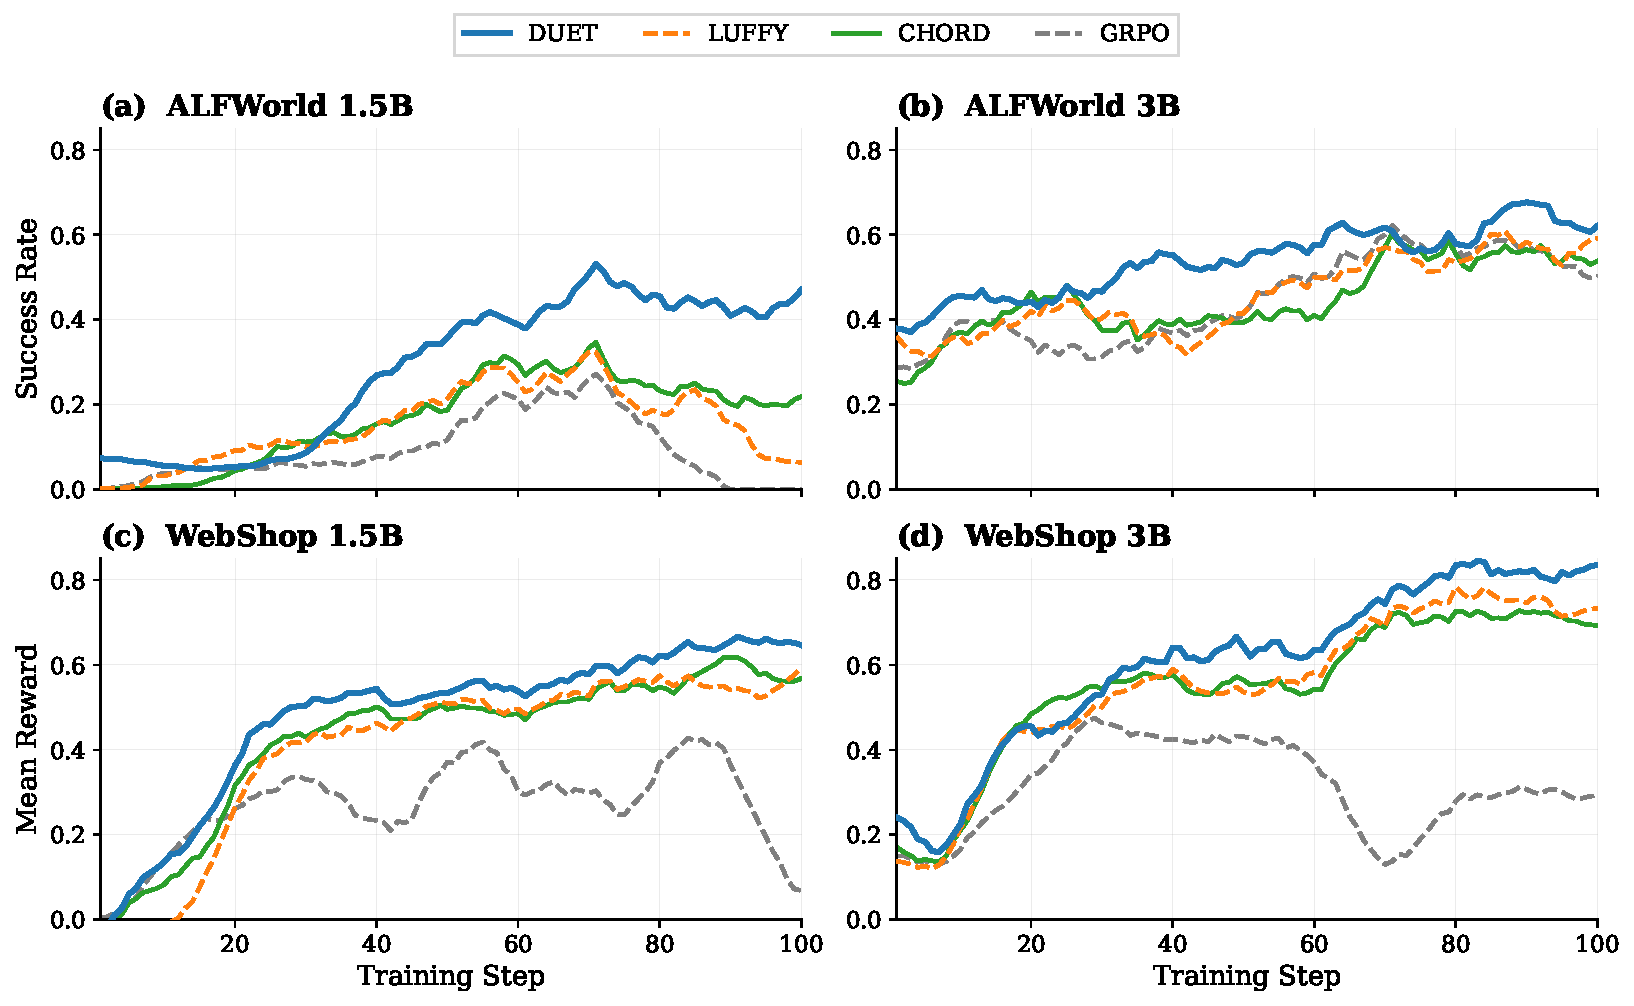
\includegraphics[width=0.99\linewidth]{figures/fig_learning_curves.pdf}%
}{%
  
\includegraphics[width=0.99\linewidth]{fig_learning_curves.pdf}%
}
\caption{
\textbf{Learning curves under the fixed 100-step budget.}
The y-axis reports on-policy success rate on ALFWorld and mean reward on WebShop.
DUET improves final performance in all four model--environment settings, with the clearest gains in the 1.5B cold-start regime.
}
\label{fig:learning_curves}
\end{figure}

\subsection{Component ablations}
\label{sec:ablations}

Table~\ref{tab:ablation} ablates DUET's components on the 1.5B settings, where cold start makes the differences most visible.
Each row removes one component while keeping the rest of the configuration fixed.

\begin{table}[t]
\centering
\caption{
\textbf{Component ablations on 1.5B students.}
Each row removes one DUET component while keeping all others fixed.
The rightmost column reports the average drop from full DUET across the two environments.
}
\label{tab:ablation}
\resizebox{0.92\linewidth}{!}{
\begin{tabular}{llccc}
\toprule
Variant & Component removed & 1.5B-AF & 1.5B-WS & Avg. $\Delta$ \\
\midrule
DUET (full) & -- & 47.5\% & 36.0\% & -- \\
w/o baseline sep. & Advantage normalization & 0.0\%$^\star$ & 0.0\%$^\star$ & $-41.8$pp \\
w/o DR3 weighting & Density-ratio correction & 38.5\% & 9.5\% & $-17.8$pp \\
w/o State Channel & Progress reward shaping & 31.0\% & 1.0\% & $-25.8$pp \\
w/o BC & Cold-start imitation & 34.0\% & 16.5\% & $-16.5$pp \\
\midrule
OnPolicy GRPO & No teacher data & 1.0\% & 0.5\% & -- \\
\bottomrule
\end{tabular}
}
\vspace{0.3em}
\begin{flushleft}
{\footnotesize $^\star$ Training collapses to 0\% within the first $\sim$50 steps when baseline separation is removed.}
\end{flushleft}
\end{table}

\paragraph{Baseline separation is critical.}
Removing baseline separation collapses both 1.5B settings to 0.0\%, making it the largest ablation effect.
This matches the failure mode predicted by Eq.~\eqref{eq:baseline_contamination}: without separation, high-reward teacher trajectories shift the baseline upward and suppress credit for rare successful on-policy rollouts.

\paragraph{Visualizing the contamination bias.}
Figure~\ref{fig:advantage_distribution} shows per-trajectory advantage distributions on 1.5B-ALFWorld at three training stages, with and without baseline separation.
With baseline separation, the on-policy mean stays near zero throughout training ($\mu_{\rm on}=0.06,0.05,0.04$).
Without it, the on-policy distribution drifts negative as teacher rewards raise the shared baseline ($\mu_{\rm on}=0.02\rightarrow -0.04\rightarrow -0.17$).
This matches the sign and direction predicted by Eq.~\eqref{eq:baseline_contamination}, and provides a direct visual explanation for the collapse observed in Table~\ref{tab:ablation}.

\begin{figure}[t]
\centering
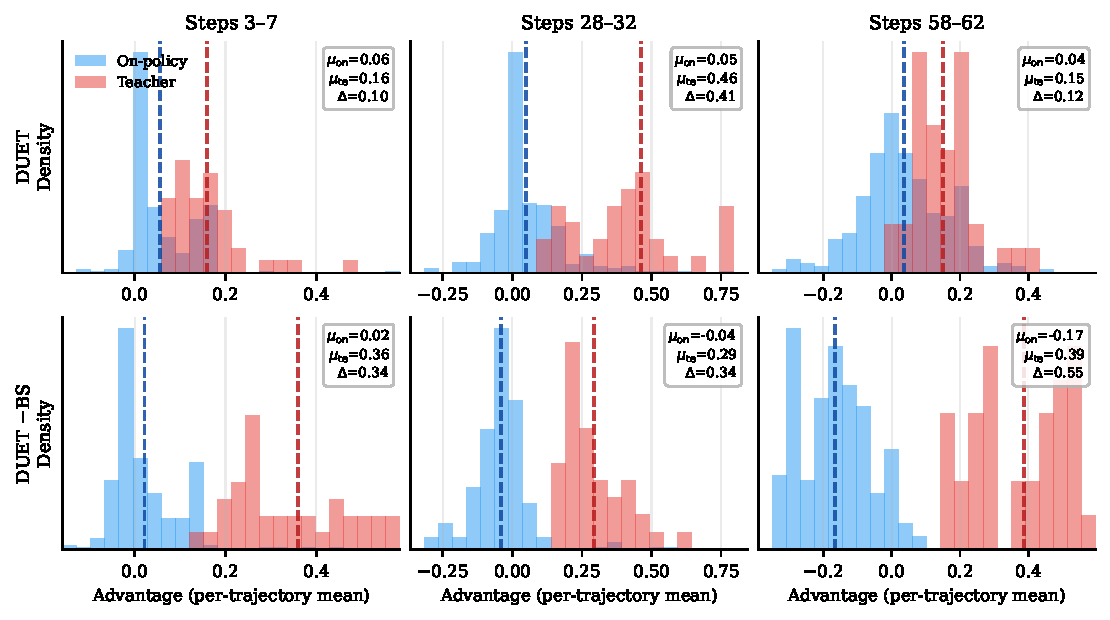
\includegraphics[width=0.86\linewidth]{figures/fig_advantage_dist.pdf}
\caption{
\textbf{Advantage distributions with and without baseline separation} on 1.5B-ALFWorld.
Top row: full DUET; on-policy means stay near zero throughout training.
Bottom row: DUET with baseline separation removed; on-policy means drift negative as teacher rewards inflate the shared GRPO baseline, in the direction predicted by Eq.~\eqref{eq:baseline_contamination}.
}
\label{fig:advantage_distribution}
\end{figure}

\paragraph{Different components address different failure modes.}
Removing the State Channel reduces performance by 16.5pp on ALFWorld and 35.0pp on WebShop, showing that progress-based shaping provides substantial exploration guidance.
Removing DR3 causes a significant drop on both environments, suggesting that distribution correction matters most when the teacher--student gap persists over longer or more diverse interactions.
Behavior cloning also contributes in both environments by providing dense cold-start supervision before the discriminator-based correction stabilizes.

\subsection{Action Channel dynamics}
\label{sec:dynamics}

The Action Channel is designed to reduce teacher influence according to training signals rather than a fixed step schedule.
Figure~\ref{fig:dynamics} reports the quantities that control this behavior.
The effective teacher replay weight decreases over training, the BC coefficient decays from its cold-start value, and discriminator accuracy rises above chance.
Together, these trends indicate that DUET relies most strongly on teacher actions early in training and gradually attenuates their effect.

\begin{figure}[t]
\centering
\IfFileExists{figures/fig3_self_attenuation.pdf}{%
  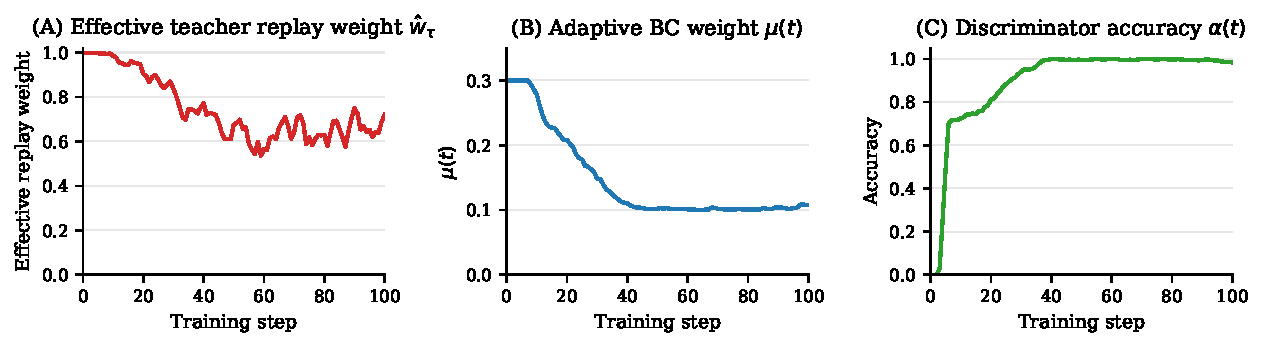
\includegraphics[width=0.86\linewidth]{figures/fig3_self_attenuation.pdf}%
}{%
  
\includegraphics[width=0.86\linewidth]{fig3_self_attenuation.pdf}%
}
\caption{
\textbf{Self-attenuation in the Action Channel.}
(A) The effective teacher replay weight $\hat{w}_\tau$ decreases over training.
(B) The adaptive behavior-cloning coefficient $\mu(t)$ decays after the cold-start phase.
(C) Discriminator accuracy $\alpha(t)$ rises above chance, providing the signal used to attenuate teacher-action influence.
}
\label{fig:dynamics}
\end{figure}

\paragraph{Two complementary fade-out paths.}
DUET reduces teacher influence through two signals.
The first comes from asymmetric baseline separation: by Eq.~\eqref{eq:teacher_advantage}, the teacher centered reward is proportional to $(1-p_o)$, so it shrinks as on-policy success improves.
The second comes from DR3: $\hat w$ tracks the teacher--student distribution gap and decreases as teacher samples become easier to distinguish from on-policy samples.
These mechanisms respond to reward progress and distributional progress, respectively, allowing teacher influence to recede without a fixed step-indexed schedule.

% ============================================================================
% Main Results Table — DUET* vs External Baselines
% 4 settings: 1.5B AlfWorld, 1.5B WebShop, 3B AlfWorld, 3B WebShop
% Metric: val@100 success rate (strict, score >= 1.0)
% ============================================================================
%
% Required packages (add to preamble of neurips_2026.tex):
%   \usepackage{booktabs}
%   \usepackage{multirow}
%   \usepackage{xcolor}
%   \usepackage[table]{xcolor}
%
% Usage in main.tex:
%   % ============================================================================
% Main Results Table — DUET* vs External Baselines
% 4 settings: 1.5B AlfWorld, 1.5B WebShop, 3B AlfWorld, 3B WebShop
% Metric: val@100 success rate (strict, score >= 1.0)
% ============================================================================
%
% Required packages (add to preamble of neurips_2026.tex):
%   \usepackage{booktabs}
%   \usepackage{multirow}
%   \usepackage{xcolor}
%   \usepackage[table]{xcolor}
%
% Usage in main.tex:
%   % ============================================================================
% Main Results Table — DUET* vs External Baselines
% 4 settings: 1.5B AlfWorld, 1.5B WebShop, 3B AlfWorld, 3B WebShop
% Metric: val@100 success rate (strict, score >= 1.0)
% ============================================================================
%
% Required packages (add to preamble of neurips_2026.tex):
%   \usepackage{booktabs}
%   \usepackage{multirow}
%   \usepackage{xcolor}
%   \usepackage[table]{xcolor}
%
% Usage in main.tex:
%   \input{tables/main_results.tex}
% ============================================================================

\begin{table}[t]
\centering
\caption{Main results: \textbf{DUET\textsuperscript{*} achieves SOTA across all four (model size $\times$ environment) settings}, surpassing the strongest baseline by an average of \textbf{+13.0pp} success rate at val@100. All numbers are strict success rate ($\text{score} \geq 1.0$, val@100). Best per column in \textbf{bold}; second-best \underline{underlined}. Improvements ($\Delta$) computed against the strongest non-DUET baseline.}
\label{tab:main_results}
\setlength{\tabcolsep}{6pt}
\renewcommand{\arraystretch}{1.15}
\begin{tabular}{lcccc}
\toprule
\textbf{Method} & \textbf{1.5B-ALFWorld} & \textbf{1.5B-WebShop} & \textbf{3B-ALFWorld} & \textbf{3B-WebShop} \\
\midrule
OnPolicy GRPO       & 1.0\%             & 0.5\%             & 47.0\%            & 2.0\%$^\dagger$   \\
SFT (no RL)         & ---               & 7.0\%             & ---               & ---               \\
LUFFY               & 5.5\%             & 5.5\%             & 61.5\%            & 38.0\%            \\
CHORD               & 27.0\%            & 11.5\%            & \underline{67.0\%} & \underline{39.0\%} \\
SFT $+$ GRPO        & \underline{30.0\%} & \underline{18.5\%} & 59.5\%            & 24.0\%            \\
\midrule
\rowcolor{gray!12}
\textbf{DUET\textsuperscript{*} (Ours)} & \textbf{47.5\%} & \textbf{36.0\%} & \textbf{77.5\%} & \textbf{45.5\%} \\
\midrule
$\Delta$ over best baseline & $+17.5$pp & $+17.5$pp & $+10.5$pp & $+6.5$pp \\
\bottomrule
\end{tabular}
\vspace{2pt}

\raggedright
\footnotesize
$^\dagger$ OnPolicy GRPO collapses on 3B-WebShop without expert guidance.
\end{table}

% ============================================================================

\begin{table}[t]
\centering
\caption{Main results: \textbf{DUET\textsuperscript{*} achieves SOTA across all four (model size $\times$ environment) settings}, surpassing the strongest baseline by an average of \textbf{+13.0pp} success rate at val@100. All numbers are strict success rate ($\text{score} \geq 1.0$, val@100). Best per column in \textbf{bold}; second-best \underline{underlined}. Improvements ($\Delta$) computed against the strongest non-DUET baseline.}
\label{tab:main_results}
\setlength{\tabcolsep}{6pt}
\renewcommand{\arraystretch}{1.15}
\begin{tabular}{lcccc}
\toprule
\textbf{Method} & \textbf{1.5B-ALFWorld} & \textbf{1.5B-WebShop} & \textbf{3B-ALFWorld} & \textbf{3B-WebShop} \\
\midrule
OnPolicy GRPO       & 1.0\%             & 0.5\%             & 47.0\%            & 2.0\%$^\dagger$   \\
SFT (no RL)         & ---               & 7.0\%             & ---               & ---               \\
LUFFY               & 5.5\%             & 5.5\%             & 61.5\%            & 38.0\%            \\
CHORD               & 27.0\%            & 11.5\%            & \underline{67.0\%} & \underline{39.0\%} \\
SFT $+$ GRPO        & \underline{30.0\%} & \underline{18.5\%} & 59.5\%            & 24.0\%            \\
\midrule
\rowcolor{gray!12}
\textbf{DUET\textsuperscript{*} (Ours)} & \textbf{47.5\%} & \textbf{36.0\%} & \textbf{77.5\%} & \textbf{45.5\%} \\
\midrule
$\Delta$ over best baseline & $+17.5$pp & $+17.5$pp & $+10.5$pp & $+6.5$pp \\
\bottomrule
\end{tabular}
\vspace{2pt}

\raggedright
\footnotesize
$^\dagger$ OnPolicy GRPO collapses on 3B-WebShop without expert guidance.
\end{table}

% ============================================================================

\begin{table}[t]
\centering
\caption{Main results: \textbf{DUET\textsuperscript{*} achieves SOTA across all four (model size $\times$ environment) settings}, surpassing the strongest baseline by an average of \textbf{+13.0pp} success rate at val@100. All numbers are strict success rate ($\text{score} \geq 1.0$, val@100). Best per column in \textbf{bold}; second-best \underline{underlined}. Improvements ($\Delta$) computed against the strongest non-DUET baseline.}
\label{tab:main_results}
\setlength{\tabcolsep}{6pt}
\renewcommand{\arraystretch}{1.15}
\begin{tabular}{lcccc}
\toprule
\textbf{Method} & \textbf{1.5B-ALFWorld} & \textbf{1.5B-WebShop} & \textbf{3B-ALFWorld} & \textbf{3B-WebShop} \\
\midrule
OnPolicy GRPO       & 1.0\%             & 0.5\%             & 47.0\%            & 2.0\%$^\dagger$   \\
SFT (no RL)         & ---               & 7.0\%             & ---               & ---               \\
LUFFY               & 5.5\%             & 5.5\%             & 61.5\%            & 38.0\%            \\
CHORD               & 27.0\%            & 11.5\%            & \underline{67.0\%} & \underline{39.0\%} \\
SFT $+$ GRPO        & \underline{30.0\%} & \underline{18.5\%} & 59.5\%            & 24.0\%            \\
\midrule
\rowcolor{gray!12}
\textbf{DUET\textsuperscript{*} (Ours)} & \textbf{47.5\%} & \textbf{36.0\%} & \textbf{77.5\%} & \textbf{45.5\%} \\
\midrule
$\Delta$ over best baseline & $+17.5$pp & $+17.5$pp & $+10.5$pp & $+6.5$pp \\
\bottomrule
\end{tabular}
\vspace{2pt}

\raggedright
\footnotesize
$^\dagger$ OnPolicy GRPO collapses on 3B-WebShop without expert guidance.
\end{table}
  % placeholder so Table~1 can be referenced now

% ============================================================================
% Section 5: Discussion / Limitations
% TODO: discuss
%   - Single-seed caveat
%   - LUFFY reproducibility
%   - When DUET helps most (cold-start regime)
% ============================================================================
% % ============================================================================
% Discussion and Limitations
% ============================================================================

\section{Discussion and Limitations}
\label{sec:discussion}

\paragraph{When DUET helps most.}
DUET is designed for the regime where teacher replay is most useful but also most likely to bias the update: sparse-reward training with weak student policies.
In this regime, the on-policy reward stream contains few successful rollouts, so teacher trajectories provide necessary guidance.
At the same time, directly mixing high-reward teacher rollouts into GRPO can distort the group baseline and over-emphasize off-policy actions.
The empirical results follow this pattern: DUET gives its largest gains on the 1.5B students, where on-policy GRPO nearly collapses, and smaller but still positive gains on the 3B students, where the on-policy stream is already more informative.

\paragraph{Which components are load-bearing.}
The ablations suggest that the components play different roles.
Baseline separation is the most consistently important mechanism: removing it collapses both 1.5B settings, matching the baseline-contamination failure mode analyzed in Section~\ref{sec:action_channel}.
The State Channel provides dense exploration guidance and is especially helpful when task progress can be inferred from intermediate observations.
DR3 is more environment-dependent.
It has a large effect on WebShop, where the teacher--student mismatch persists over longer and more diverse interactions, but a smaller marginal effect on ALFWorld, where baseline separation and cold-start imitation already close much of the gap.
This suggests that DUET should be viewed as a framework for separating teacher signals, rather than as a claim that every component contributes equally in every environment.

\paragraph{Dependence on teacher data.}
DUET assumes access to a cache of successful teacher trajectories.
The quality, diversity, and filtering of this cache can affect all three sources of teacher influence: the action replay signal, the density-ratio estimate, and the state-progress map.
A narrow teacher cache may bias the State Channel toward a limited set of solution paths, while a noisy or weak teacher cache may provide unreliable progress signals.
Our experiments use successful trajectories from a stronger teacher model, which matches the intended cold-start setting but does not cover cases where teacher demonstrations are suboptimal, heterogeneous, or adversarially filtered.

\paragraph{Limits of the current density-ratio correction.}
Our DR3 implementation estimates a trajectory-level replay weight and applies it uniformly to the teacher tokens in that trajectory.
This is a coarse approximation.
A token-level or step-level density ratio could focus the correction on teacher actions that are unlikely under the current student, and might reduce the need for a separate behavior-cloning bridge.
We leave this finer-grained correction to future work.

\paragraph{Limits of the State Channel.}
The State Channel relies on matching on-policy observations to states seen in successful teacher trajectories.
This works naturally in environments where progress can be recognized from textual observations or structured attributes, but it may be less reliable when observations are highly aliased, noisy, or only weakly correlated with task completion.
In such settings, a learned progress model or uncertainty-aware shaping rule may be needed.

\paragraph{Scope of evaluation.}
Our evaluation focuses on two representative interactive LLM-agent settings: embodied text interaction and web navigation. 
These settings capture sparse rewards, multi-turn interaction, and teacher-guided cold start, which are the main conditions DUET is designed for. 
The magnitude of the gains may vary with horizon length, teacher quality, and how much progress information is exposed in the environment state.


% ============================================================================
% Section 6: Conclusion
% TODO
% ============================================================================
% % ============================================================================
% Conclusion — DUET (NeurIPS 2026)
% ============================================================================

\section{Conclusion}
\label{sec:conclusion}

We studied teacher replay for reinforcement learning of LLM agents under GRPO-style training. 
Although teacher trajectories provide valuable cold-start signal, directly mixing them with on-policy rollouts can bias group-relative advantage estimation and leave teacher-action gradients uncorrected when teacher likelihoods are unavailable. 
DUET addresses these issues with two complementary uses of teacher data: corrected action-level replay through baseline separation and density-ratio weighting, and state-level guidance through progress-based reward shaping. 
Experiments on ALFWorld and WebShop show that DUET improves over teacher-replay and imitation-based baselines across student model scales, especially when the student has little initial on-policy success. 
We hope this perspective encourages future work to treat teacher demonstrations as structured interaction traces, rather than only as action sequences to imitate.


% ============================================================================
% Acknowledgements (hidden in anonymous submission via 'ack' env)
% ============================================================================
\begin{ack}
% Funding and competing-interest disclosures go here for the camera-ready.
% Required by NeurIPS 2026:
%   https://neurips.cc/Conferences/2026/PaperInformation/FundingDisclosure
\end{ack}


% ============================================================================
% References
% TODO: switch to bibtex once .bib file is set up. For now, manual entries.
% ============================================================================
\section*{References}

\medskip

{
\small

% --- Placeholder bibtex keys used in section files (TODO: bibtex) ---
% TODO_grpo       — Shao et al. (2024). DeepSeekMath / GRPO.
% TODO_luffy      — LUFFY (cite original work).
% TODO_chord      — CHORD (cite original work).
% TODO_alfworld   — Shridhar et al. (2021). ALFWorld.
% TODO_webshop    — Yao et al. (2022). WebShop.
% TODO_react      — Yao et al. (2023). ReAct.
% TODO_ng1999     — Ng, Harada \& Russell (1999). Policy invariance under reward
%                   transformations: theory and application to reward shaping.

[1]~Placeholder reference --- to be replaced with bibtex entries.

}


%%%%%%%%%%%%%%%%%%%%%%%%%%%%%%%%%%%%%%%%%%%%%%%%%%%%%%%%%%%%

\appendix

\section{Technical appendices and supplementary material}
% TODO: appendix sections will include:
%   - LUFFY reproducibility study (3.5\% / 38.0\% / 49.5\% three-way comparison)
%   - Hyperparameter sensitivity tables
%   - Additional training-dynamics figures
%   - Implementation details

%%%%%%%%%%%%%%%%%%%%%%%%%%%%%%%%%%%%%%%%%%%%%%%%%%%%%%%%%%%%

\newpage
\input{checklist.tex}


\end{document}
